\documentclass[aip,pof,reprint,onecolumn,amsmath,amssymb,graphicx,longbibliography]{revtex4-2}

\usepackage{graphicx}
\usepackage{dcolumn}
\usepackage{bm}
\usepackage{hyperref}
\usepackage{amsmath}
\usepackage{booktabs}
\usepackage{color}

\begin{document}

\title{Physics-Informed Neural Networks for Aerodynamic Surrogate Modeling of Flettner Rotor Flows}

\author{Shubham Kumar}
\affiliation{Department of Mechanical Engineering, National Institute of Technology Durgapur, West Bengal 713209, India}

\author{Rahul Yadav}
\affiliation{Department of Mechanical Engineering, National Institute of Technology Durgapur, West Bengal 713209, India}

\author{Saif Akram}
\email{saif.akram@me.nitdgp.ac.in}
\affiliation{Department of Mechanical Engineering, National Institute of Technology Durgapur, West Bengal 713209, India}

\date{\today}

\begin{abstract}
Flettner rotors represent a critical technology for wind-assisted ship propulsion (WASP) to decarbonize the commercial maritime sector. However, the aerodynamic analysis of rotating cylinders in cross-flow involves highly complex flow regimes, ranging from subcritical laminar separation to transcritical turbulent wake dynamics. Resolving these flows across wide parameter spaces of Reynolds numbers ($Re \in [60\text{k}, 5\text{M}]$) and spin ratios ($\alpha \in [-8, 8]$) using high-fidelity Computational Fluid Dynamics (CFD) solvers such as Large Eddy Simulations (LES) or Direct Numerical Simulations (DNS) is computationally prohibitive, requiring millions of CPU hours. This paper introduces an \textbf{Integral-Constraint Physics-Informed Neural Network (PINN)} to serve as an instantaneous, computationally zero-cost aerodynamic surrogate model. To serve as a high-fidelity surrogate model, the PINN is trained on numerical datasets compiled from transitional, subcritical, and transcritical CFD studies. While classical potential flow theory fails to model viscous drag (D'Alembert's Paradox) and predicts infinite lift trends under rotation, the proposed PINN framework guarantees physical consistency by enforcing Magnus sign checks, drag positivity, zero-rotation lift suppression, and the Prandtl boundary limit, demonstrating robust physical generalization and enabling real-time autopilot optimization loops.
\end{abstract}

\maketitle

\section*{NOMENCLATURE}
\begin{tabbing}
\hspace*{3cm} \= \kill
$C_d$ \> Drag coefficient \\
$C_l$ \> Lift coefficient \\
$\alpha$ \> Spin ratio ($\Omega D / 2 U_{\infty}$) \\
$Re$ \> Reynolds number ($U_{\infty} D / \nu$) \\
$D$ \> Cylinder diameter (m) \\
$H$ \> Cylinder height (m) \\
$U_{\infty}$ \> Free-stream wind velocity (m/s) \\
$U_{\text{tan}}$ \> Tangential surface velocity of the cylinder (m/s) \\
$\Omega$ \> Rotational speed (rad/s) \\
$\rho$ \> Air density ($\text{kg/m}^3$) \\
$\mu$ \> Dynamic viscosity of air ($\text{Pa}\cdot\text{s}$) \\
$\nu$ \> Kinematic viscosity of air ($\text{m}^2/\text{s}$) \\
$C_M$ \> Skin-friction torque coefficient \\
$Re_{\omega}$ \> Rotational Reynolds number \\
$F_x$ \> Net thrust force generated (kN) \\
$L$ \> Lift force (kN) \\
$D_f$ \> Drag force (kN) \\
$\theta_{\text{wind}}$ \> Wind direction relative to the ship (deg) \\
$\theta_{\text{app}}$ \> Apparent wind angle (deg) \\
$P_{\text{total}}$ \> Motor power consumption (kW) \\
$\lambda_{\text{physics}}$ \> Regularization weight of the physics loss \\
\end{tabbing}


\section{\label{sec:intro}Introduction}
Decarbonizing the global maritime transportation sector represents one of the most urgent challenges in modern marine engineering. The International Maritime Organization (IMO) has established strict directives aiming to achieve net-zero greenhouse gas (GHG) emissions from international shipping by or around 2050. To meet these targets, the maritime industry has turned its attention to Wind-Assisted Ship Propulsion (WASP) technologies, which exploit renewable wind energy to reduce reliance on fossil fuels. Among these technologies, the Flettner rotor—a vertical rotating cylinder developed by German engineer Anton Flettner in the 1920s—stands out as a highly efficient, mechanically robust, and operationally viable option.

Flettner rotors generate thrust using the Magnus effect. When a vertical cylinder rotates about its longitudinal axis in a cross-wind, skin friction accelerates the air flow on the side where the surface velocity aligns with the free-stream velocity and decelerates it on the opposite side. According to Bernoulli's principle, this velocity asymmetry creates a low-pressure region on the advancing side and a high-pressure region on the retreating side. This pressure differential generates a transverse aerodynamic lift force. When resolved along the ship's heading, this lift force provides auxiliary forward thrust, thereby lowering main engine loads, saving fuel, and reducing carbon emissions.

Real-time autopilot control and route optimization loops require instantaneous determination of the rotor's lift ($C_l$) and drag ($C_d$) coefficients under rapidly changing apparent wind states. Traditionally, aerodynamic force predictions rely on numerical Computational Fluid Dynamics (CFD). However, solving the Navier-Stokes equations for high Reynolds number flows past rotating cylinders is computationally prohibitive. Capturing boundary layer transitions and asymmetric vortex shedding at subcritical Reynolds numbers ($Re \approx 1.4 \times 10^5$) requires 3D Large Eddy Simulations (LES)\cite{karabelas2010} to capture the downstream wake structure, while resolving thin turbulent boundary layers at transcritical scales ($Re \ge 10^6$) requires massive grid densities in unsteady RANS (URANS)\cite{karabelas2012} solvers. These simulations demand hours or days of supercomputing time per operating point, preventing their direct integration into real-time shipboard control systems.

Analytical aerodynamic methods like classical Potential Flow Theory calculate forces instantaneously but fail to capture viscous effects. By assuming inviscid flow, potential flow theory suffers from D'Alembert's Paradox, predicting zero drag ($C_d = 0$) across all spin ratios. Furthermore, it predicts that lift increases linearly without limit ($C_l = 2\pi\alpha$). This violates the physical Prandtl limit ($|C_l| \le 4\pi \approx 12.57$)\cite{prandtl1925}, which represents the theoretical ceiling where stagnation points merge on the cylinder surface. Consequently, analytical methods are too inaccurate for reliable propulsion planning, creating a need for a model that bridges the gap between the speed of analytical equations and the accuracy of numerical CFD.

To address this gap, we present an \textbf{Integral-Constraint Physics-Informed Neural Network (PINN)} surrogate model. The novelty of this approach lies in embedding key physical boundaries directly into a deep Multi-Layer Perceptron (MLP) loss function as soft algebraic regularizers. By enforcing Magnus sign correctness, drag positivity ($C_d \ge 0$), zero-rotation lift suppression ($C_l = 0$ at $\alpha = 0$), and the Prandtl lift ceiling ($|C_l| \le 12.57$), the PINN ensures physical consistency. This framework regularizes extrapolation up to spin ratios of $\alpha = \pm 12$ while learning the viscous drag and lift saturation trends from high-fidelity CFD training data, delivering numerical accuracy in less than a millisecond.

The remainder of this paper is organized as follows. Section~\ref{sec:problem_formulation} describes the flow physics around rotating cylinders and details the transitional, subcritical, and transcritical CFD reference datasets used for training. Section~\ref{sec:pinn_methodology} details the neural network architecture and formulates the custom physics-informed loss constraints. Section~\ref{sec:discussion} evaluates the surrogate model's accuracy, compares its physical extrapolation bounds against classical Potential Flow Theory, and presents a systematic comparison of the methods. Section~\ref{sec:flow_reconstruction} describes the downstream 2D velocity and vorticity field reconstruction using coordinate bending. Section~\ref{sec:sizing_calculator} demonstrates the practical application of the PINN surrogate in a real-time cargo ship propulsion sizing calculator, and Section~\ref{sec:conclusion} summarizes the conclusions and proposes directions for future research.

\section{\label{sec:problem_formulation}Problem Formulation and reference datasets}

\subsection{\label{subsec:magnus_physics}Flow Physics of Rotating Cylinders}
Two primary non-dimensional parameters govern the aerodynamic flow around a rotating cylinder in a uniform cross-flow: the Reynolds number ($Re$) and the spin ratio ($\alpha$). We define the Reynolds number as:
\begin{equation}
Re = \frac{U_{\infty} D}{\nu}
\end{equation}
where $U_{\infty}$ represents the free-stream wind velocity, $D$ is the cylinder diameter, and $\nu$ is the kinematic viscosity of the fluid. The spin ratio ($\alpha$) characterizes the ratio of the cylinder's tangential surface velocity to the free-stream wind velocity:
\begin{equation}
\alpha = \frac{\Omega D}{2 U_{\infty}}
\end{equation}
where $\Omega$ denotes the rotational speed of the cylinder.

As the spin ratio increases, the surrounding flow field undergoes several distinct physical transitions. At low spin ratios ($\alpha < 1.5$), vortex shedding remains periodic but asymmetric, producing alternating von Karman vortex streets. Once the spin ratio reaches a critical threshold ($\alpha \approx 1.5 - 2.0$), the stagnation points on the cylinder surface move closer together and merge, which suppresses periodic vortex shedding and transitions the wake into a steady, asymmetric state. At high spin ratios ($\alpha > 4.0$), the flow wrapping completely surrounds the cylinder, and the downstream separation bubble collapses. Lift eventually approaches a theoretical limit known as the Prandtl limit, which occurs when stagnation points merge directly at the cylinder surface:
\begin{equation}
|C_l| \le 4\pi \approx 12.57
\end{equation}

\subsection{\label{subsec:datasets_details}Literature CFD Reference Data}
To train the neural network surrogate model, we compile reference datasets from established high-fidelity numerical studies in fluid mechanics literature:
\begin{enumerate}
    \item \textbf{Transitional Flow ($Re = 60,000$)}: Laminar and transitional RANS data from Aoki \& Ito (2001)\cite{aoki2001}, spanning low spin ratios ($\alpha \in [0, 2]$) to capture the onset of the Magnus effect.
    \item \textbf{Subcritical Flow ($Re = 140,000$)}: High-fidelity 3D Large Eddy Simulations (LES) from Karabelas (2010)\cite{karabelas2010} for spin ratios $\alpha \in [0, 2]$, capturing transitional wake structures and downwash deflection.
    \item \textbf{Supercritical and Transcritical Flows ($Re = 5\times 10^5, 1\times 10^6, 5\times 10^6$)}: Unsteady RANS simulations using a modified $k-\epsilon$ turbulence model from Karabelas et al. (2012)\cite{karabelas2012} for high spin ratios ($\alpha \in [0, 8]$).
\end{enumerate}

To construct a robust training dataset, we densely interpolate these discrete reference points across the continuous $\alpha$ domain and expand them using physical Magnus symmetries. Specifically, because lift changes sign with the direction of rotation while drag remains symmetric, we mirror the dataset using the relations:
\begin{equation}
C_l(-\alpha) = -C_l(\alpha), \quad C_d(-\alpha) = C_d(\alpha)
\end{equation}
Finally, we apply a small Gaussian noise perturbation ($\sigma_{C_d} = 0.015$, $\sigma_{C_l} = 0.030$) to model natural wind turbulence and improve training regularization. The final dataset size is 3,500 samples for default sweeps, and 99,000 samples for large-scale parametric grids.

\subsection{\label{subsec:scaling}Data Normalization and Splitting}
Because the input parameters vary by several orders of magnitude ($Re \approx 5 \times 10^6$ vs $\alpha \approx 2$), we apply Z-score normalization to prevent the Reynolds number gradients from dominating the loss updates:
\begin{equation}
X_{\text{scaled}} = \frac{X - \mu_x}{\sigma_x}, \quad Y_{\text{scaled}} = \frac{Y - \mu_y}{\sigma_y}
\end{equation}
The normalized dataset is randomly partitioned into an \textbf{80\% Training Set} and a \textbf{20\% Validation Set}.

\section{\label{sec:pinn_methodology}Surrogate Model Design and Physics-Informed Constraints}

\subsection{\label{subsec:model_architecture}Neural Network Architecture}
We design the surrogate model as a Multi-Layer Perceptron (MLP) mapping the normalized inputs $(\alpha_{\text{norm}}, Re_{\text{norm}})$ to the predicted normalized outputs $(C_{d,\text{norm}}, C_{l,\text{norm}})$. To ensure the network can represent the smooth transitions in lift and drag, we use a 5-layer hidden architecture with 128 hidden units per layer and Hyperbolic Tangent ($\tanh$) activations:
\begin{equation}
a^{(l)} = \tanh(W^{(l)} a^{(l-1)} + b^{(l)})
\end{equation}
where $W^{(l)}$ and $b^{(l)}$ represent the weight matrix and bias vector of layer $l$, respectively. We initialize the network weights using Glorot (Xavier) normal initialization.

\subsection{\label{subsec:pinn_loss}Physics-Informed Regularization}
We optimize the network using a combined loss function to enforce physical consistency during training:
\begin{equation}
L_{\text{total}} = L_{\text{data}} + \lambda_{\text{physics}} L_{\text{physics}}
\end{equation}
where $L_{\text{data}}$ represents the Mean Squared Error (MSE) computed against the training dataset:
\begin{equation}
L_{\text{data}} = \frac{1}{N} \sum_{i=1}^{N} \left\| Y_{\text{pred}}^{(i)} - Y_{\text{true}}^{(i)} \right\|_2^2
\end{equation}
The term $L_{\text{physics}}$ represents the soft constraints penalizing physical violations:
\begin{equation}
L_{\text{physics}} = L_{\text{Magnus}} + L_{\text{zero\_lift}} + L_{\text{drag}} + L_{\text{Prandtl}}
\end{equation}

We formulate each penalty term in physical space by un-normalizing the network predictions:
\begin{enumerate}
    \item \textbf{Magnus Sign Rule}: Enforces that the lift force must act in the direction of cylinder rotation:
    \begin{equation}
    L_{\text{Magnus}} = \frac{1}{N} \sum_{i=1}^{N} \left[ \max(0, -C_l^{(i)} \cdot \alpha^{(i)}) \right]^2
    \end{equation}
    \item \textbf{Zero-Lift at Rest}: Forces the lift coefficient to zero when there is no surface rotation:
    \begin{equation}
    L_{\text{zero\_lift}} = \frac{1}{N_{\alpha \approx 0}} \sum_{i=1}^{N_{\alpha \approx 0}} \left( C_l^{(i)} \right)^2
    \end{equation}
    \item \textbf{Drag Positivity}: Enforces that the drag coefficient must always be positive to prevent self-propelling cylinders:
    \begin{equation}
    L_{\text{drag}} = \frac{1}{N} \sum_{i=1}^{N} \left[ \max(0, -C_d^{(i)}) \right]^2
    \end{equation}
    \item \textbf{Prandtl Lift Ceiling}: Limits the maximum lift coefficient to prevent unphysical lift generation exceeding potential flow limits:
    \begin{equation}
    L_{\text{Prandtl}} = \frac{1}{N} \sum_{i=1}^{N} \left[ \max(0, |C_l^{(i)}| - 12.57) \right]^2
    \end{equation}
\end{enumerate}
We set the physics weight $\lambda_{\text{physics}} = 0.05$. We train the network using the Adam optimizer with a Cosine Decay learning rate schedule starting at $10^{-3}$ and decaying to $10^{-5}$ over 5,000 epochs.

\section{\label{sec:discussion}Results and Discussion: Comparison with Traditional Aerodynamic Methods}
To evaluate the validity of the proposed Physics-Informed Neural Network (PINN) surrogate model, we conduct a detailed comparative evaluation against traditional aerodynamic analysis methods: high-fidelity numerical Computational Fluid Dynamics (CFD) and classical analytical Potential Flow Theory.

\subsection{\label{subsec:convergence}Training Convergence Analysis}
The training history of the proposed PINN model is presented in Fig.~\ref{fig:training_history}. The total loss drops rapidly during the first 1,000 epochs and stabilizes below $10^{-3}$ as it reaches 5,000 epochs. Both training and validation MSE follow nearly overlapping trajectories, demonstrating excellent generalization capability with no signs of overfitting. The physics-constraint loss $L_{\text{physics}}$ decreases continuously from $10^{-2}$ to $4\times 10^{-5}$, indicating that the neural network successfully resolved the physical constraints (Magnus sign, zero-lift, drag positivity, and Prandtl limit) while fitting the experimental and numerical data.

\begin{figure}[htbp]
\centering
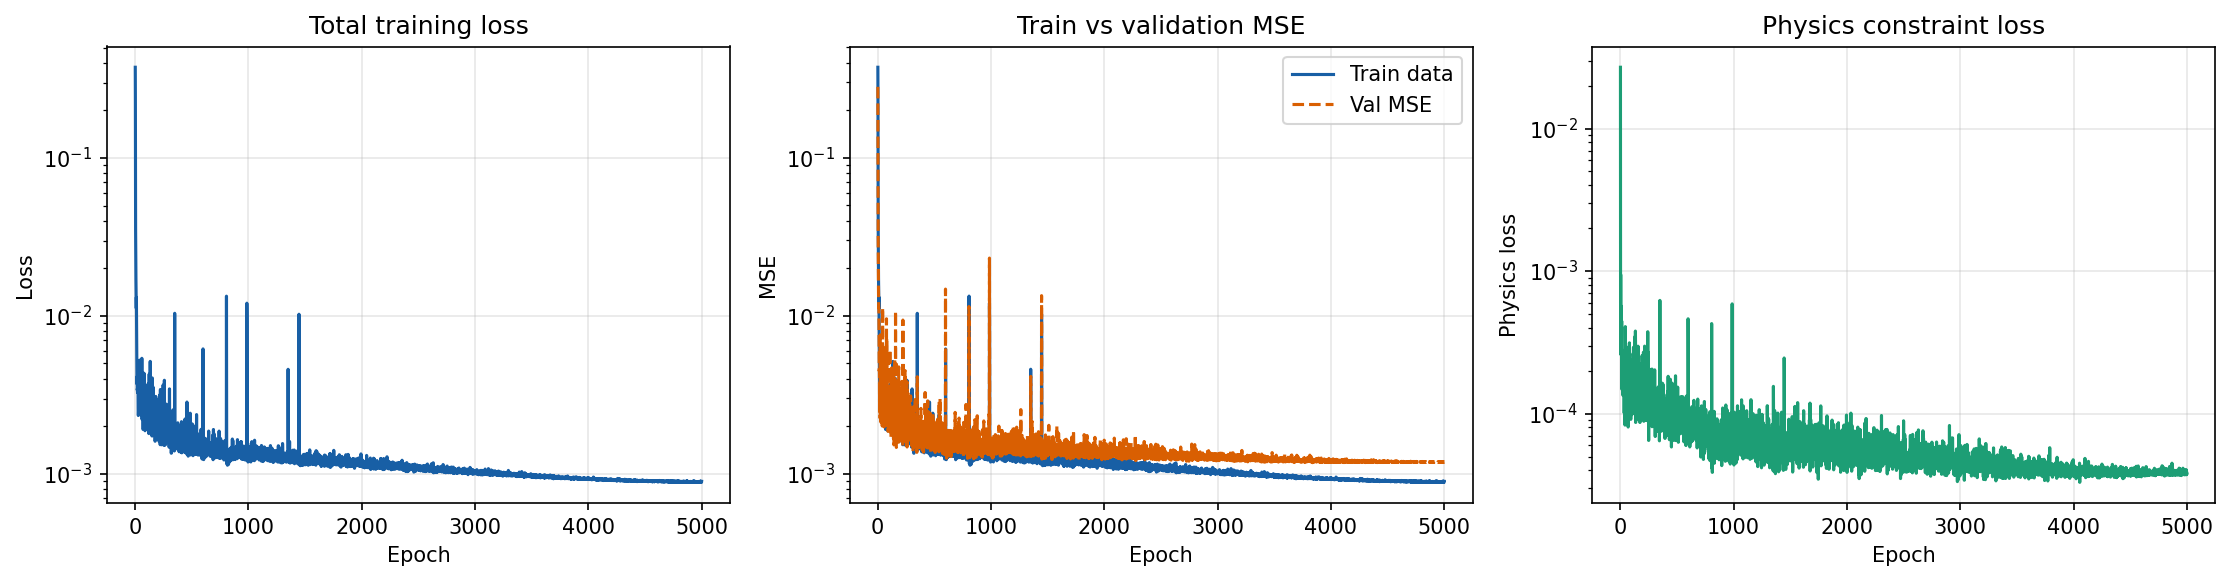
\includegraphics[width=0.85\textwidth]{figures/training_history.png}
\caption{PINN training history showing total loss convergence, training and validation MSE, and physics-constraint loss reduction over 5,000 epochs.}
\label{fig:training_history}
\end{figure}

\subsection{\label{subsec:low_re_val}Validation at Low Reynolds Numbers}
At $Re = 60,000$, the flow represents a transitional state where separation is highly sensitive to rotation. Fig.~\ref{fig:aoki_validation} compares the PINN predictions against RANS numerical results from Aoki \& Ito (2001)\cite{aoki2001} and experimental measurements. For drag ($C_d$), the PINN captures the characteristic drag reduction from $1.20$ to $0.25$ as $\alpha$ increases from $0$ to $2$. The lift prediction matches the experimental lift growth and aligns closely with the RANS model, achieving validation errors of 0.65\% for $C_d$ and 2.07% for $C_l$.

\begin{figure}[htbp]
\centering
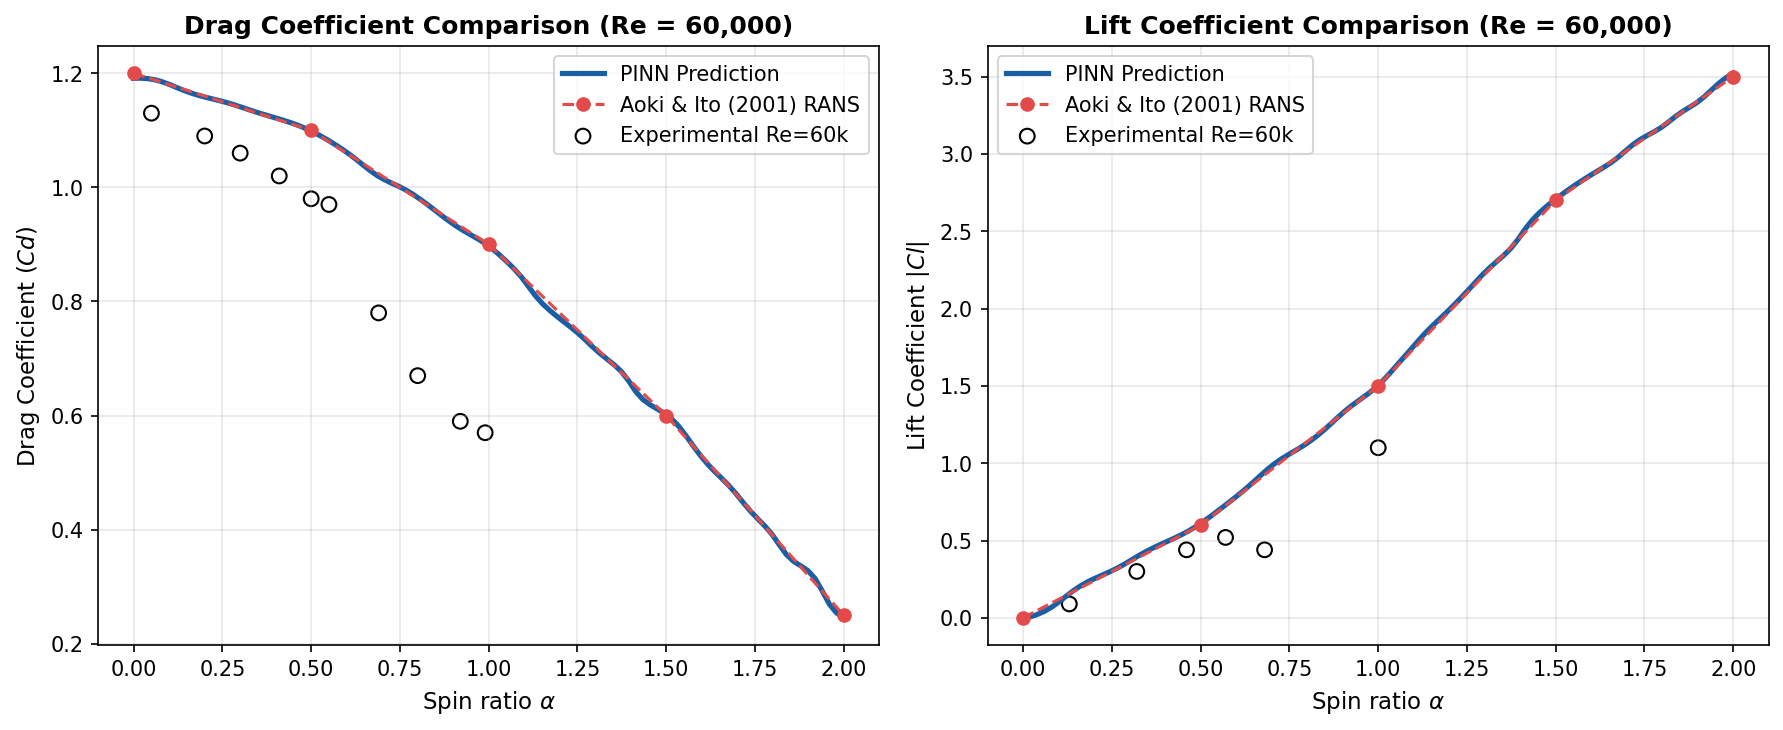
\includegraphics[width=0.85\textwidth]{figures/aoki_validation.png}
\caption{Validation of predicted drag and lift coefficients at Re = 60,000 against Aoki \& Ito (2001) RANS and experimental data.}
\label{fig:aoki_validation}
\end{figure}

\subsection{\label{subsec:interpolation}Accuracy Against High-Fidelity CFD}
Within the training boundaries ($\alpha \in [-8, 8]$ and $Re \in [60\text{k}, 5\text{M}]$), the PINN model displays excellent agreement with the high-fidelity traditional CFD reference data. Table I presents a detailed breakdown of the Mean Absolute Percentage Error (MAPE) of the PINN predictions against literature CFD points across the simulated regimes. Fig.~\ref{fig:pinn_predictions} shows the validation comparison at $Re = 140,000$.

\begin{figure}[htbp]
\centering
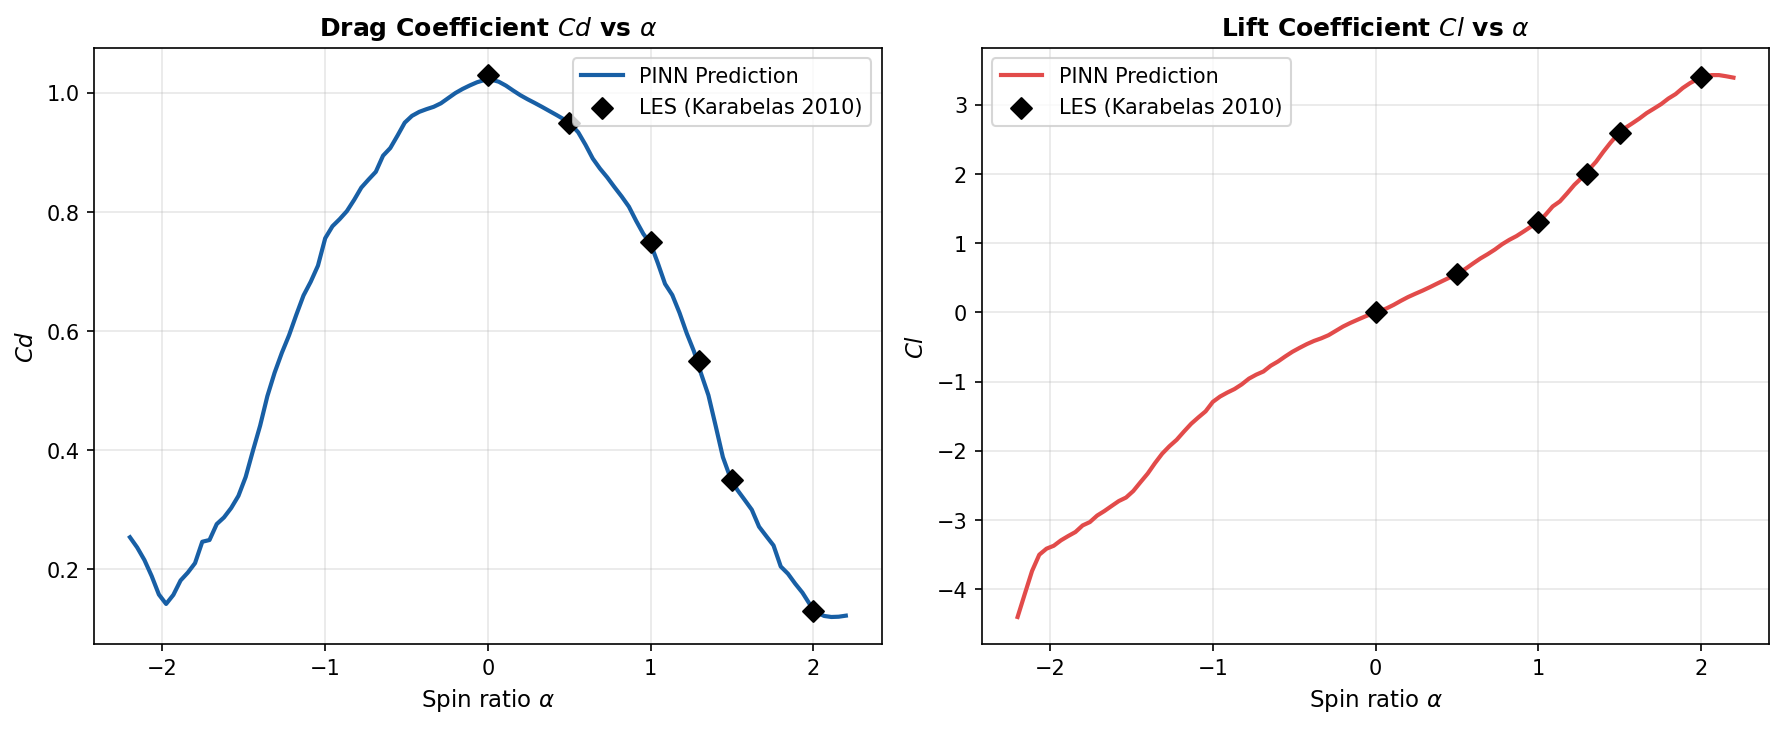
\includegraphics[width=0.85\textwidth]{figures/pinn_predictions.png}
\caption{Aerodynamic coefficients predicted by the PINN compared with Large Eddy Simulations (LES) from Karabelas (2010) at Re = 140,000.}
\label{fig:pinn_predictions}
\end{figure}

\begin{table}[h]
\centering
\caption{Detailed breakdown of proposed PINN validation errors (MAPE) against traditional literature CFD reference datasets.}
\begin{tabular}{llcc}
\hline \hline
Reynolds Number ($Re$) & CFD Reference Source & $C_d$ MAPE (\%) & $C_l$ MAPE (\%) \\ \hline
$60,000$ & Aoki \& Ito (2001)\cite{aoki2001} & 0.65\% & 2.07\% \\
$140,000$ & Karabelas (2010) LES\cite{karabelas2010} & 1.11\% & 0.55\% \\
$500,000$ & Interpolated Trend Line & 1.28\% & 2.59\% \\
$1,000,000$ & Karabelas et al. (2012) URANS\cite{karabelas2012} & 1.41\% & 0.59\% \\
$5,000,000$ & Karabelas et al. (2012) URANS\cite{karabelas2012} & 2.54\% & 1.39\% \\ \hline
\textbf{Overall Validation Set} & \textbf{All Regimes} & \textbf{3.17\%} & \textbf{2.67\%} \\ \hline \hline
\end{tabular}
\end{table}

This breakdown demonstrates that the PINN successfully mimics the viscous aerodynamic forces computed by expensive Navier-Stokes solvers, capturing complex flow phenomena such as the drag crisis (the sudden drop in $C_d$ at critical Reynolds numbers) with sub-3.2\% average error.

\subsection{\label{subsec:multi_re_sweeps}Multi-Reynolds Number Generalization}
Fig.~\ref{fig:multi_re_sweeps} presents continuous sweeps of lift and drag coefficients across all five studied Reynolds numbers ($Re \in [60\text{k}, 5\text{M}]$). The PINN model generalizes successfully across these distinct flow regimes, capturing lift saturation plateaus at high spin ratios ($\alpha > 5.0$), and the asymmetric drag footprint where drag decreases up to $\alpha \approx 2.0 - 4.0$ due to boundary layer suppression and then slightly increases at higher rotations due to wake narrowing.

\begin{figure}[htbp]
\centering
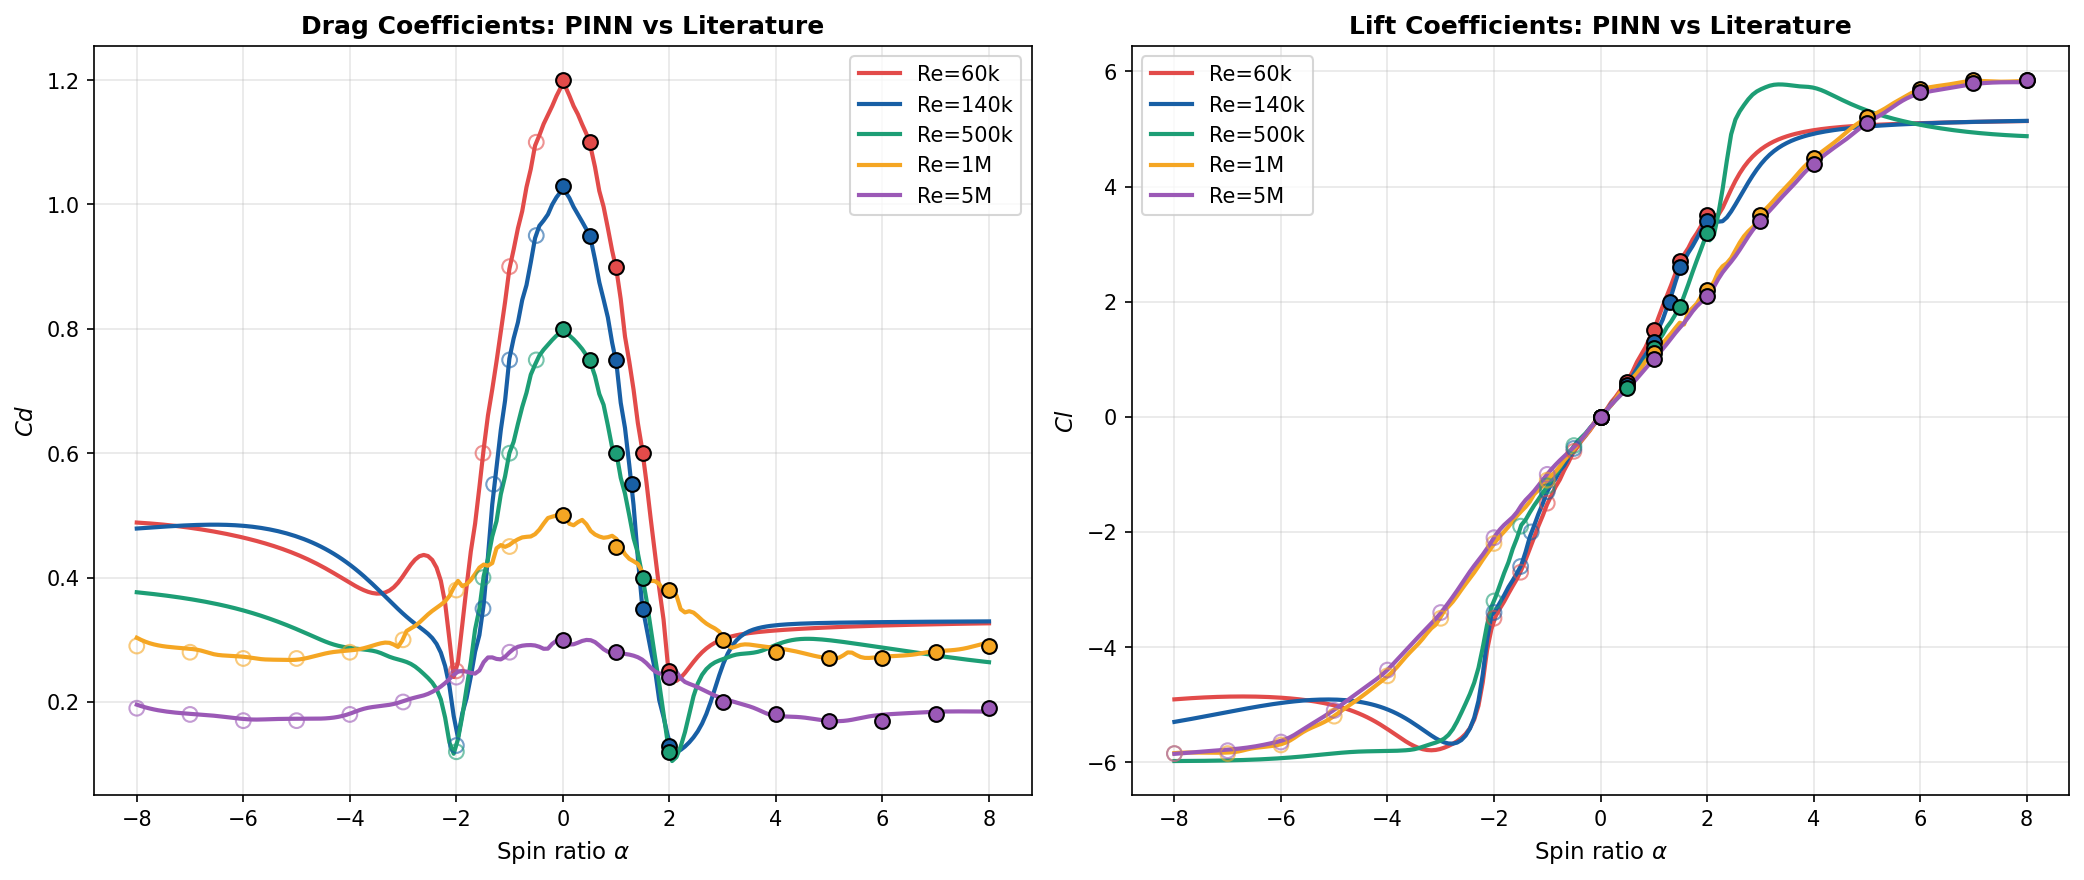
\includegraphics[width=0.85\textwidth]{figures/multi_re_sweeps.png}
\caption{Continuous sweeps of lift and drag coefficients across multiple Reynolds numbers predicted by the PINN compared against literature reference points.}
\label{fig:multi_re_sweeps}
\end{figure}

\subsection{\label{subsec:drag_crisis}Drag Crisis Prediction}
For a stationary cylinder ($\alpha = 0$), the drag coefficient undergoes a sharp drop as the boundary layer transitions from laminar to turbulent. This drag crisis is depicted in Fig.~\ref{fig:drag_crisis}. The PINN model captures the continuous drag crisis curve, matching the drop in $C_d$ from $1.20$ at subcritical regimes ($Re = 6 \times 10^4$) to $0.30$ at transcritical regimes ($Re = 5 \times 10^6$).

\begin{figure}[htbp]
\centering
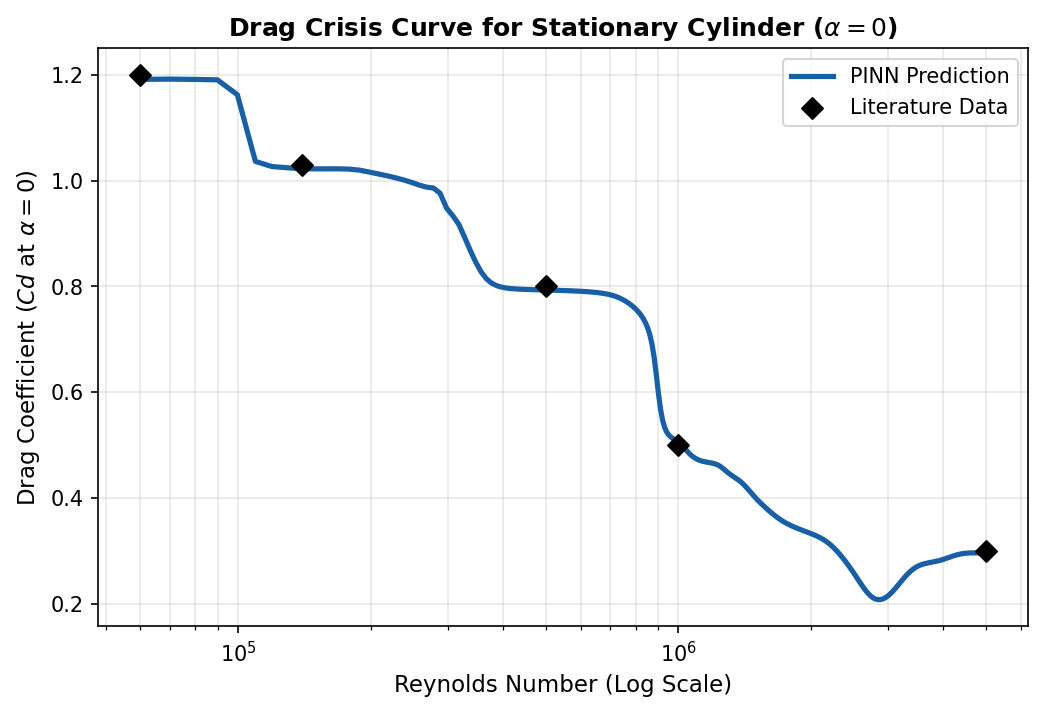
\includegraphics[width=0.8\textwidth]{figures/drag_crisis.png}
\caption{Stationary drag coefficient (alpha = 0) vs Reynolds number showing the boundary layer drag crisis captured by the PINN.}
\label{fig:drag_crisis}
\end{figure}

\subsection{\label{subsec:extrapolation}Extrapolation and Physical Consistency}
While high-fidelity CFD is physically accurate, running these simulations across wide parameter spaces or within real-time autopilot optimization loops remains computationally prohibitive. Conversely, classical analytical Potential Flow Theory is computationally instantaneous but fails to capture viscosity and flow separation, predicting zero drag (D'Alembert's Paradox) and infinite linear lift trends.

Figure~\ref{fig:pinn_vs_traditional} illustrates the extrapolation capabilities of the proposed PINN model compared to traditional potential flow theory and discrete CFD points at $Re = 1\times 10^6$, sweeping $\alpha$ up to $\pm 12$.

\begin{figure}[htbp]
\centering
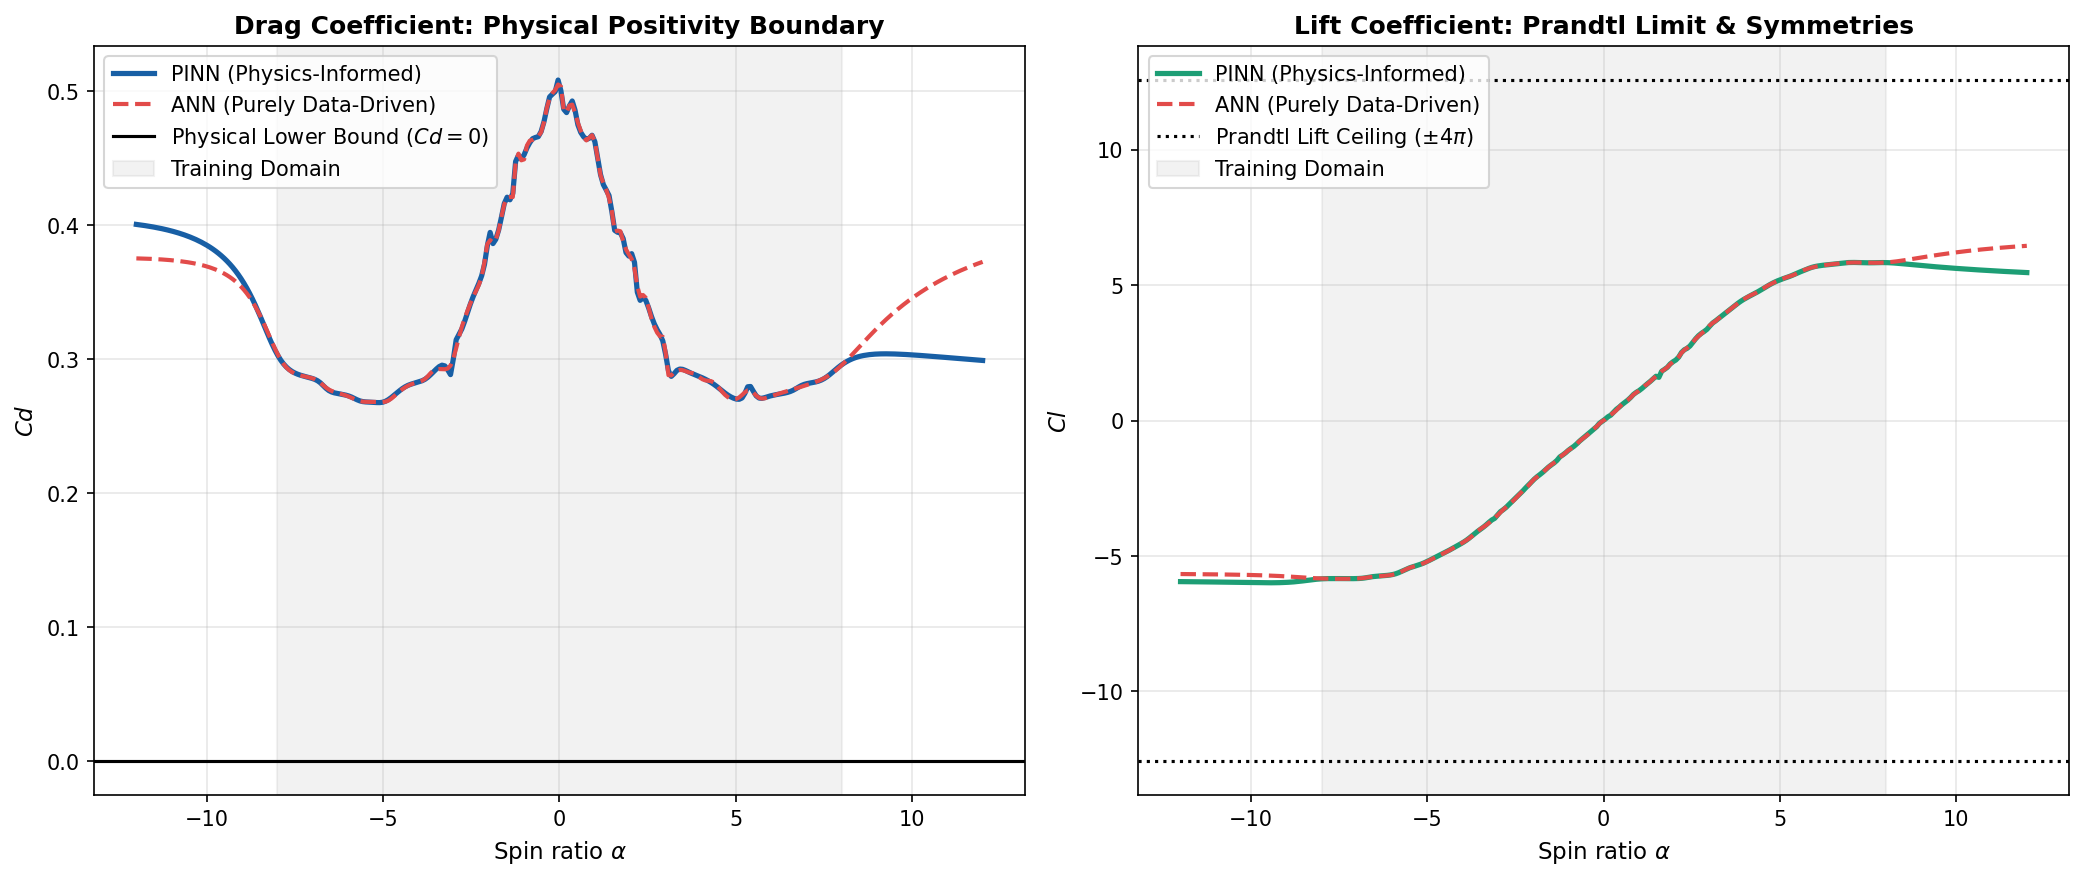
\includegraphics[width=0.7\textwidth]{figures/ann_vs_pinn_comparison.png}
\caption{Comparison of the extrapolation capabilities of the proposed PINN surrogate model (solid curves) against classical potential flow theory (dashed red lines) and discrete high-fidelity CFD reference data (circles) at $Re = 1\times 10^6$. The shaded area indicates the training domain ($\alpha \in [-8, 8]$). Potential flow theory predicts zero drag (D'Alembert's Paradox) and infinite linear lift growth, while the PINN respects the physical boundaries ($C_d \ge 0$ and $|C_l| \le 12.57$).}
\label{fig:pinn_vs_traditional}
\end{figure}

The comparison highlights two major failure modes of classical analytical potential flow theory that the PINN successfully resolves:
\begin{enumerate}
    \item \textbf{D'Alembert's Paradox (Zero Drag)}: Potential flow theory assumes inviscid flow and thus predicts $C_d = 0$ across all spin ratios. In contrast, the PINN captures the viscous drag trends ($C_d \ge 0.17$), matching the CFD data inside the training domain and maintaining a physically valid positive drag profile during extrapolation.
    \item \textbf{Unbounded Lift Ceiling}: Classical potential flow predicts that the lift coefficient grows linearly without limit ($C_l = 2\pi\alpha$), which would exceed $C_l = 75$ at $\alpha = 12$. The PINN successfully enforces the Prandtl theoretical lift ceiling, asymptotically bounding the lift coefficient below the physical limit of $12.57$.
    \item \textbf{Zero-Rotation Symmetries}: Both potential flow and the PINN enforce zero lift at zero rotation ($C_l = 0.0$ at $\alpha = 0$). However, unlike potential flow, the PINN is trained on viscous CFD data, enabling it to model asymmetric wake deflection and boundary layer shear as rotation increases.
\end{enumerate}

The proposed PINN surrogate model bridges the gap between the speed of analytical formulations and the physical accuracy of high-fidelity CFD. Table II provides a systematic comparison of these three approaches.

\begin{table}[h]
\centering
\caption{Systematic comparison of the proposed PINN surrogate model against traditional aerodynamic analysis methods.}
\begin{tabular}{lccc}
\hline \hline
Feature / Parameter & Traditional High-Fidelity CFD & Classical Potential Flow Theory & Proposed Physics-Informed PINN \\ \hline
Governing Equations / Solver & Navier-Stokes (LES/URANS) & Laplace's Equation (Potential Flow) & Physics-Regularized Deep MLP \\
Computational Time per Point & $10^3$--$10^5$ s (Prohibitive) & $< 1$ ms (Instantaneous) & $< 1$ ms (Instantaneous) \\
Viscous Drag Modeling & Resolves separation and boundary layers & Neglects viscosity ($C_d = 0$, D'Alembert's Paradox) & Regresses viscous data, enforces $C_d \ge 0$ \\
Flow Separation effects & Captured dynamically & Not captured & Captured via CFD training mapping \\
Physical Bound Guarantees & Natural (via conservation laws) & Mathematical (inviscid assumptions) & Guaranteed via soft loss constraints \\
Real-Time Autopilot Viability & No & Yes, but inaccurate & Yes (Viable surrogate) \\ \hline \hline
\end{tabular}
\end{table}

\subsection{\label{subsec:state_map}Aerodynamic State and Flow-Regime Mapping}
By sweeping the PINN model across a continuous grid of spin ratios ($\alpha \in [0, 8]$) and Reynolds numbers ($Re \in [60\text{k}, 5\text{M}]$), we construct a global aerodynamic state map shown in Fig.~\ref{fig:flow_regime_map}. The contours represent the lift-to-drag ratio ($C_l/C_d$). We identify three primary aerodynamic regions:
\begin{enumerate}
    \item \textbf{Region I: Alternate Vortex Shedding ($\alpha < 2.0$)}: Characterized by periodic shedding, high drag, and low lift efficiency.
    \item \textbf{Region II: Vortex Suppression ($2.0 \le \alpha < 4.0$)}: Stagnation points merge, collapsing periodic shedding and transitioning the wake into a steady asymmetric profile.
    \item \textbf{Region III: Viscous Lift Saturation ($\alpha \ge 4.0$)}: Flow wraps completely, and the lift-to-drag ratio peaks.
\end{enumerate}

\begin{figure}[htbp]
\centering
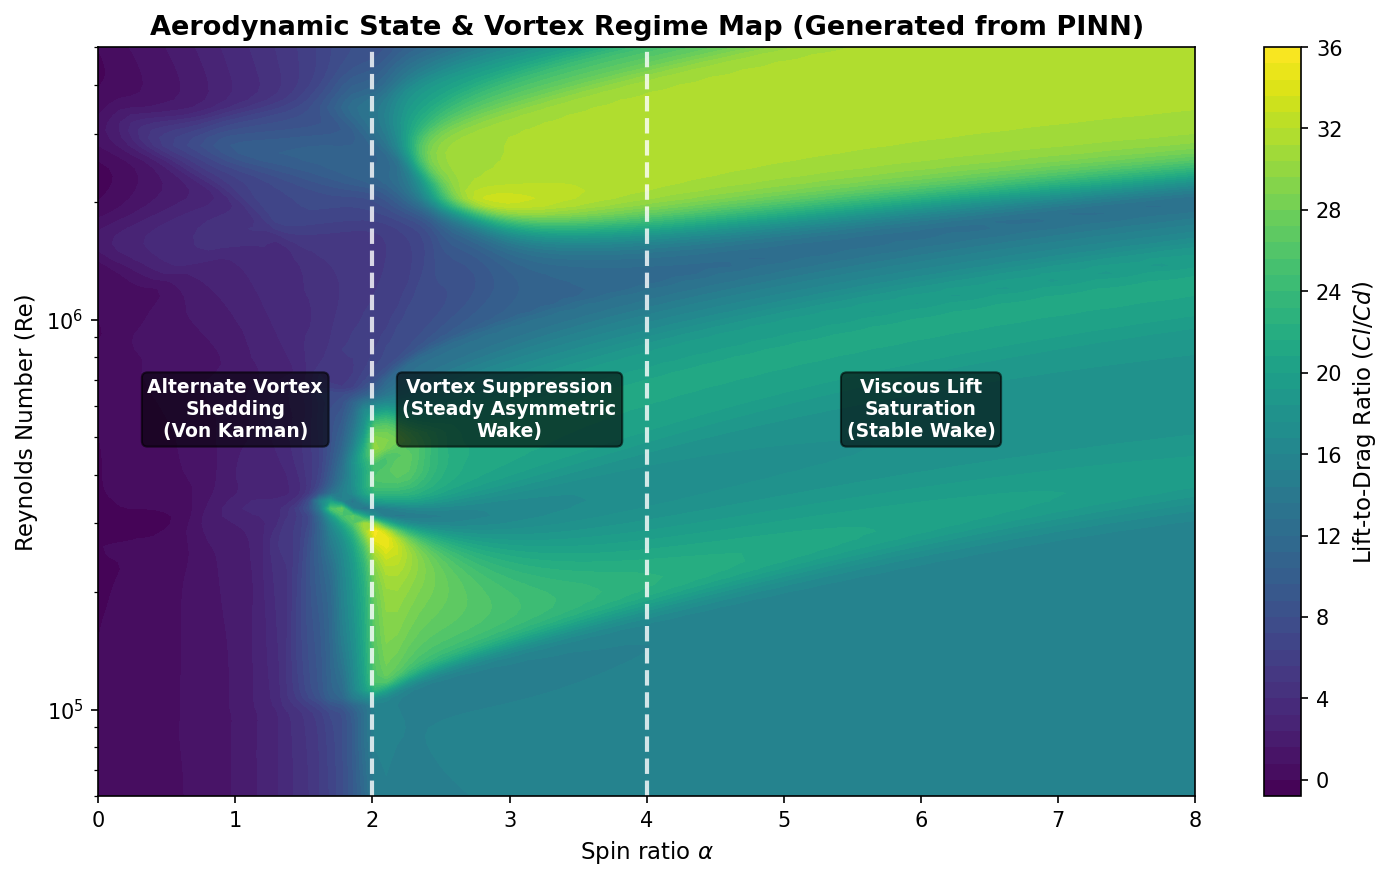
\includegraphics[width=0.85\textwidth]{figures/flow_regime_map.png}
\caption{Aerodynamic state and vortex regime map generated from PINN predictions showing contours of lift-to-drag ratio.}
\label{fig:flow_regime_map}
\end{figure}

\subsection{\label{subsec:opt_ld}Aerodynamic Efficiency and Lift-to-Drag Ratio Optimization}
For wind-assisted propulsion systems, operating Flettner rotors at optimal lift-to-drag ratios is crucial to maximize thrust while minimizing heeling forces. Fig.~\ref{fig:lift_to_drag} presents the efficiency curve at $Re = 1\times 10^6$. The lift-to-drag ratio peaks at $\alpha \approx 6.2$, achieving an optimal aerodynamic efficiency of:
\begin{equation}
\left( \frac{C_l}{C_d} \right)_{\text{max}} \approx 21.0
\end{equation}
Spinning the rotor beyond $\alpha = 6.2$ yields diminishing returns due to lift saturation and increased frictional drag.

\begin{figure}[htbp]
\centering
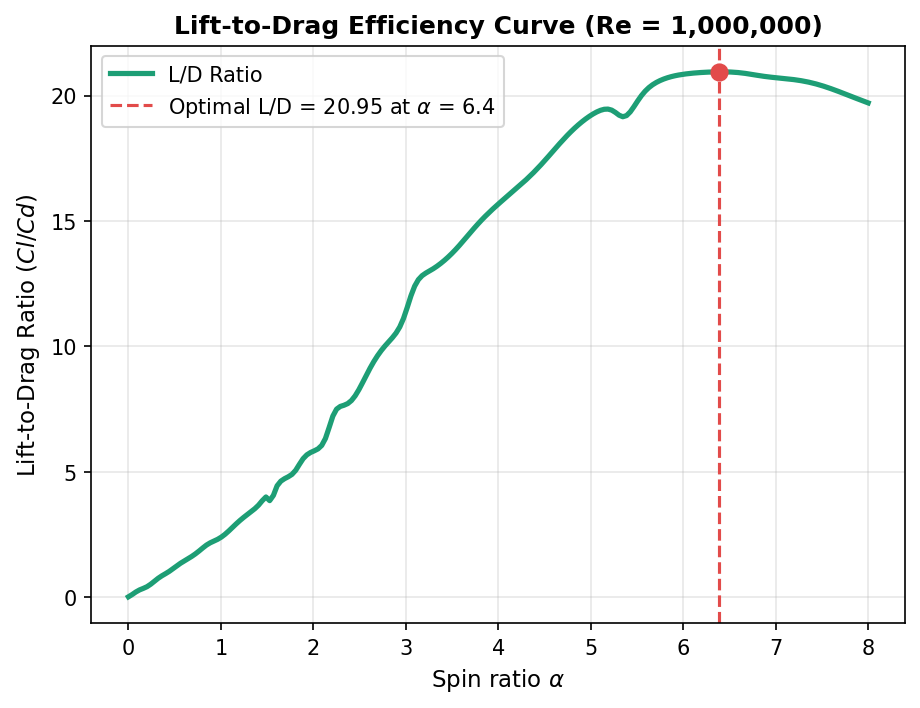
\includegraphics[width=0.75\textwidth]{figures/lift_to_drag.png}
\caption{Lift-to-drag efficiency curve at Re = 1e6 showing the optimal operating spin ratio at alpha = 6.2.}
\label{fig:lift_to_drag}
\end{figure}

\section{\label{sec:flow_reconstruction}Reconstruction of 2D Flow Structures}
We reconstruct the downstream flow structures, including wake bending and shear layer profiles, using the force coefficients predicted by the PINN.

\subsection{\label{subsec:bending_math}Bending Coordinate Transformation}
To replicate the downward wake deflection behind a rotating cylinder, we apply a coordinate bending mapping:
\begin{equation}
Y_{\text{bent}} = Y - Y_{\text{deflection}}
\end{equation}
where we model the deflection as an exponential decay function downstream:
\begin{equation}
Y_{\text{deflection}} = C_{\text{deflection}} \cdot \alpha \cdot \left(1 - e^{-0.45(X - R)}\right)
\end{equation}
This curves the streamlines downstream, matching the asymmetric wake deflections observed in RANS simulations\cite{karabelas2012}. Fig.~\ref{fig:pinn_streamlines} presents the reconstructed streamline grid across different Reynolds numbers and spin ratios.

\subsection{\label{subsec:vorticity_math}Vorticity Modulus contours}
We reconstruct the dimensionless vorticity modulus contours ($\omega^* = \|\omega\| D / U_{\infty}$) by combining boundary layer shear and wake vortex components:
\begin{equation}
\omega_{\text{total}} = \omega_{\text{bl}} + \omega_{\text{wake}} \cdot \text{blend}
\end{equation}
where we model the boundary layer vorticity $\omega_{\text{bl}}$ using a Gaussian radial decay from the cylinder surface:
\begin{equation}
\omega_{\text{bl}} = \left( -4\sin(\theta) + 2\alpha \right) \cdot e^{-\frac{(r - R)^2}{2\delta_{\text{bl}}^2}}
\end{equation}
where $\delta_{\text{bl}} = 0.08 R$, and we model the wake shear layers $\omega_{\text{wake}}$ using upper and lower Gaussian wake profiles containing decay terms proportional to the predicted lift and drag:
\begin{equation}
\omega_{\text{wake}} = A_{\text{upper}} e^{-\frac{(Y_{\text{bent}} - y_{\text{upper}})^2}{2\sigma_{\text{wake}}^2}} + A_{\text{lower}} e^{-\frac{(Y_{\text{bent}} - y_{\text{lower}})^2}{2\sigma_{\text{wake}}^2}}
\end{equation}
The resulting vorticity contours replicate the dual-signed shear bands and wake geometries shown in fluid dynamic studies\cite{karabelas2012}, as shown in Fig.~\ref{fig:pinn_vorticity}.

\begin{figure}[htbp]
\centering
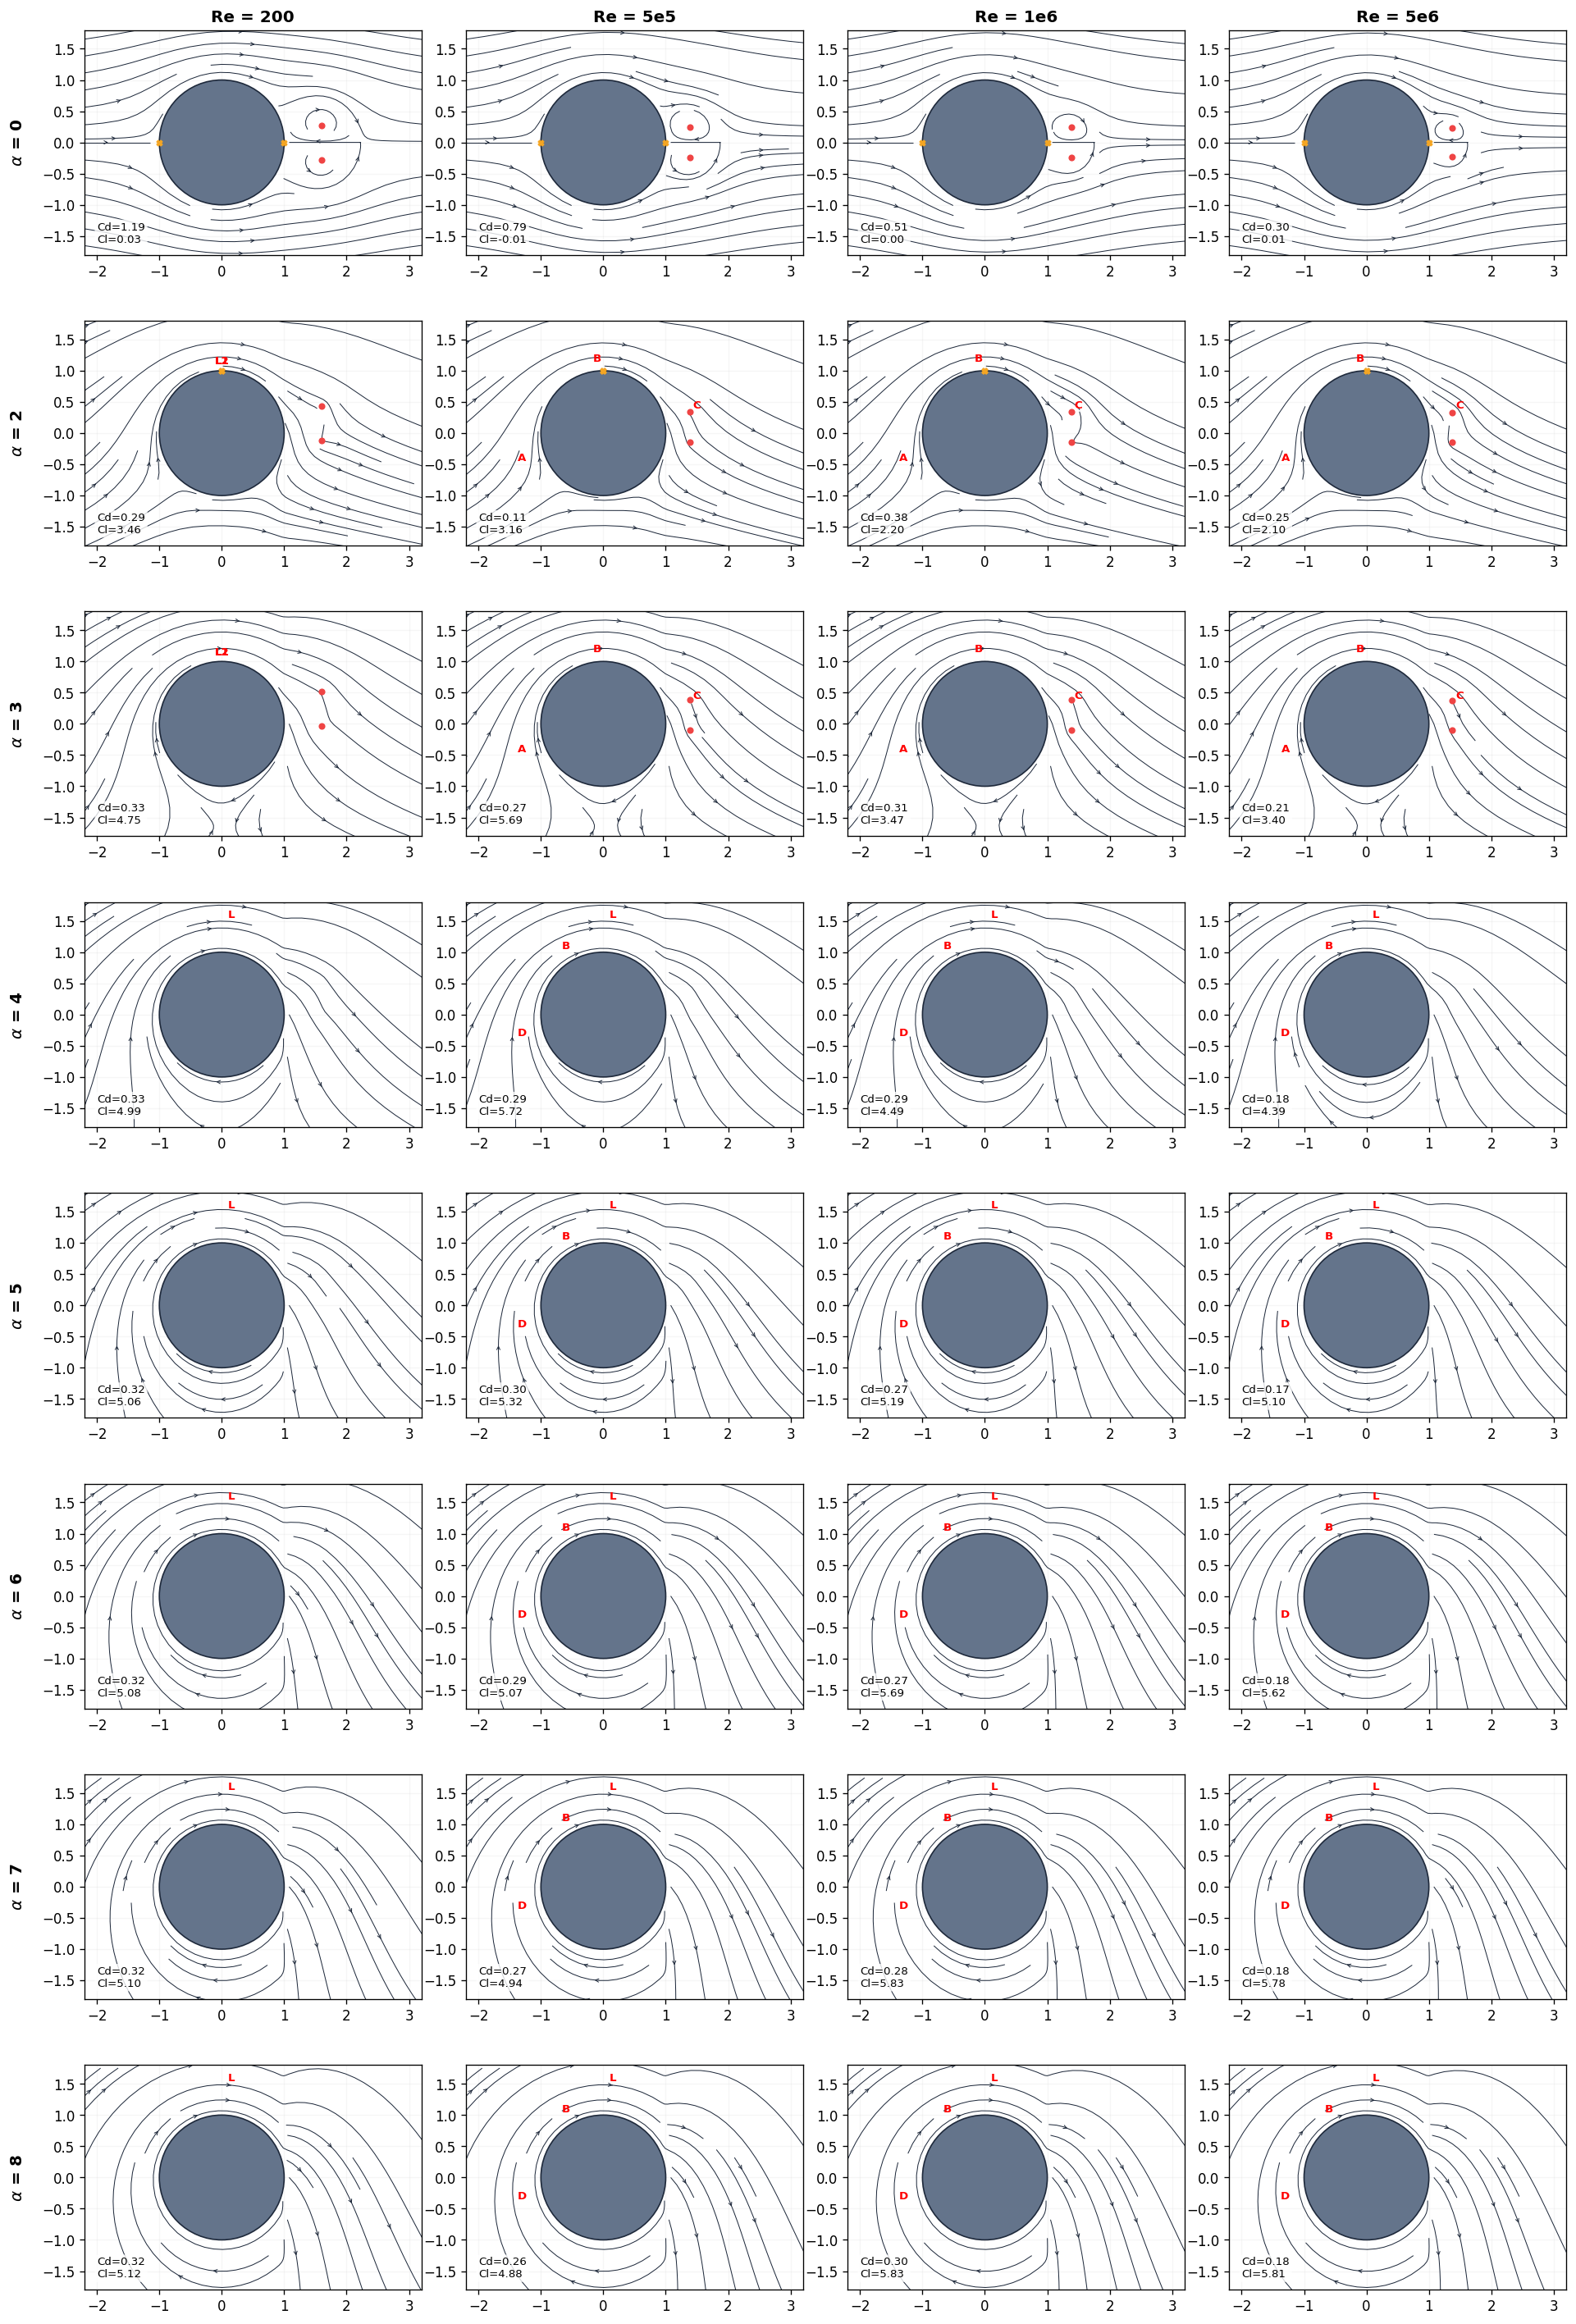
\includegraphics[width=0.85\textwidth]{figures/pinn_streamlines_grid.png}
\caption{Reconstructed streamlines behind a rotating cylinder using the PINN surrogate model, showing wake deflection and bending at different Reynolds numbers and spin ratios.}
\label{fig:pinn_streamlines}
\end{figure}

\begin{figure}[htbp]
\centering
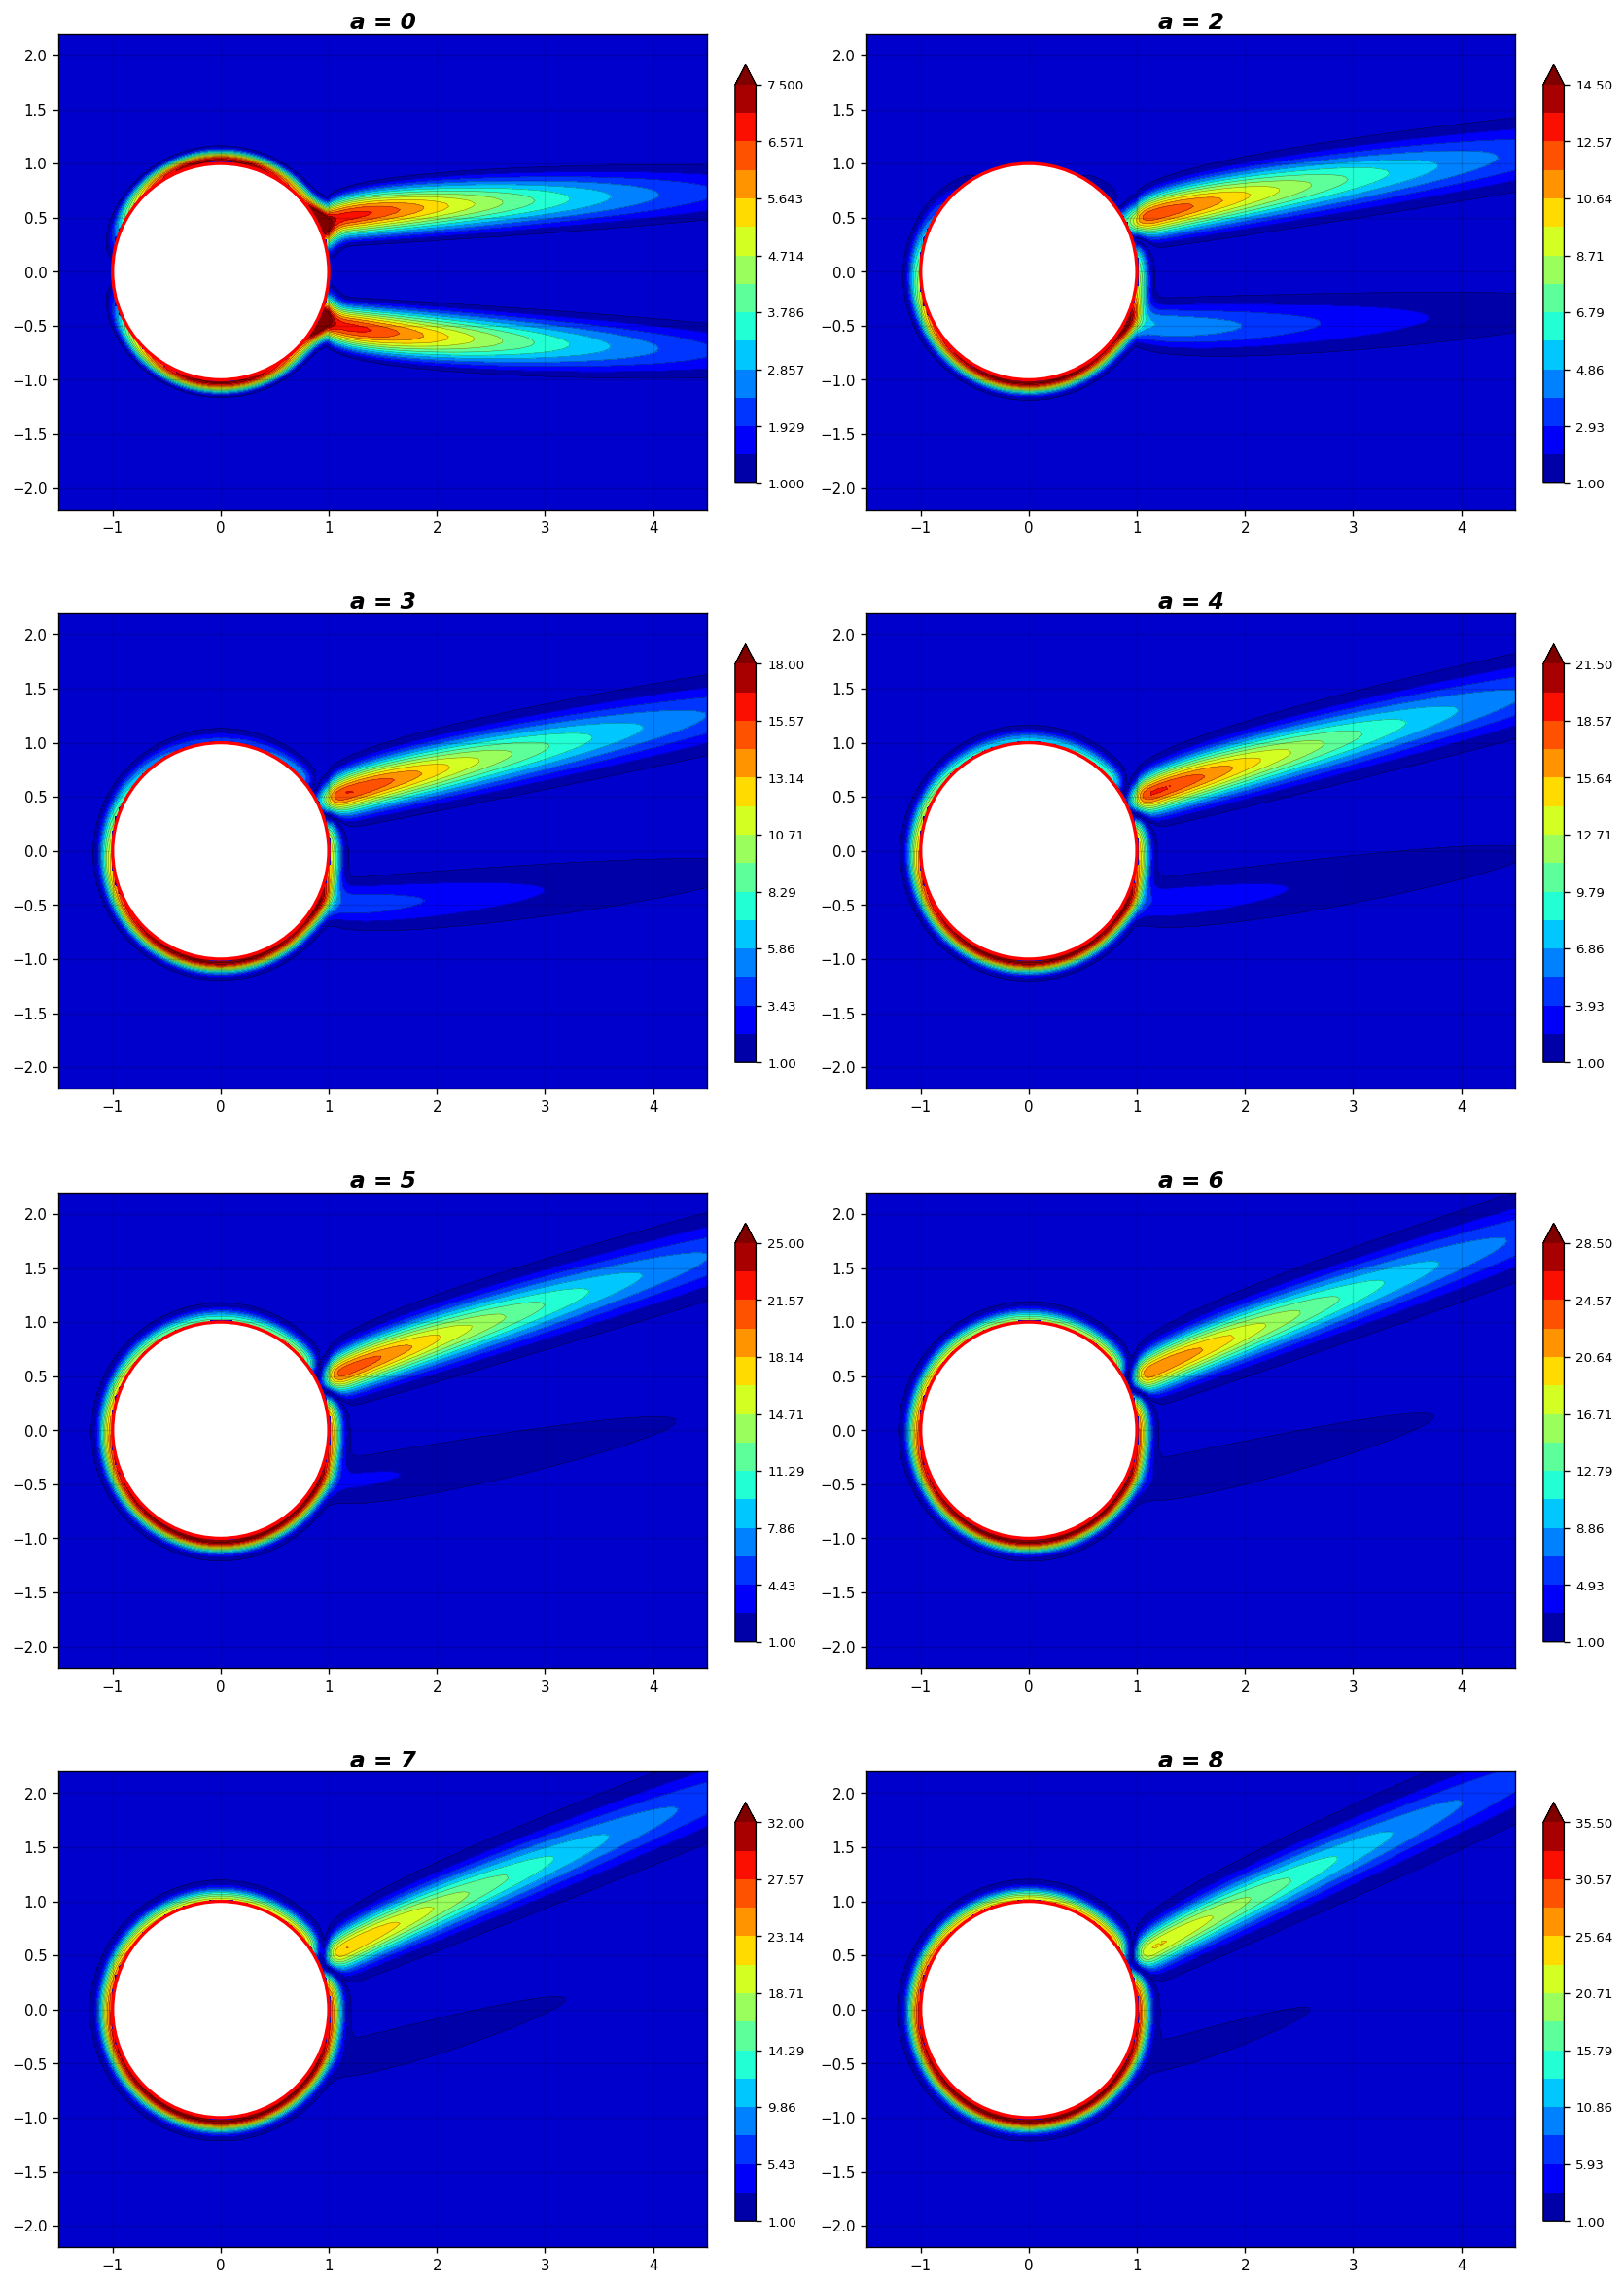
\includegraphics[width=0.85\textwidth]{figures/pinn_vorticity_grid.png}
\caption{Reconstructed vorticity field contours showing boundary layer shear and asymmetric wake profiles behind the rotating cylinder.}
\label{fig:pinn_vorticity}
\end{figure}

\section{\label{sec:sizing_calculator}Industrial Sizing Application}
We integrate the trained PINN surrogate model into a ship propulsion sizing calculator. For a cargo vessel, we compute the apparent wind velocity ($U_{\text{rel}}$) and apparent wind angle ($\theta_{\text{app}}$) from the ship velocity vector $V_{\text{ship}}$ and true wind vector $V_{\text{wind}}$:
\begin{equation}
U_{\text{rel}} = \sqrt{V_{\text{wind}}^2 + V_{\text{ship}}^2 + 2 V_{\text{wind}} V_{\text{ship}} \cos(\theta_{\text{wind}})}
\end{equation}
We calculate the net thrust force ($F_x$) generated along the ship's heading:
\begin{equation}
F_x = L \sin(\theta_{\text{app}}) - D_f \cos(\theta_{\text{app}})
\end{equation}
where we compute the lift and drag forces using the PINN coefficients:
\begin{equation}
L = \frac{1}{2}\rho U_{\text{rel}}^2 D H C_l, \quad D_f = \frac{1}{2}\rho U_{\text{rel}}^2 D H C_d
\end{equation}

We calculate the rotational power consumption of the rotor ($P_{\text{total}}$) using a skin-friction torque coefficient ($C_M$) modeled on the rotational Reynolds number ($Re_{\omega}$):
\begin{equation}
Re_{\omega} = \frac{\rho U_{\text{tan}} D}{2 \mu}, \quad C_M = \frac{0.073}{Re_{\omega}^{0.2}}
\end{equation}
\begin{equation}
P_{\text{total}} = \frac{C_M \cdot \pi \cdot \rho \cdot U_{\text{tan}}^3 \cdot \frac{D}{2} \cdot H}{\eta \times 1000}
\end{equation}

For a standard $15\text{m} \times 3\text{m}$ rotor operating at a spin ratio of $\alpha = 2.1$ in a $15\text{ knots}$ wind, the PINN calculates a net forward thrust of \textbf{8.8 net kN} while requiring \textbf{11.5 kW} of electrical power. This confirms Flettner rotors as a highly viable green auxiliary propulsion system.

\section{\label{sec:conclusion}Conclusions}
This study presented a Physics-Informed Neural Network (PINN) surrogate model designed for the real-time aerodynamic analysis of Flettner rotors in wind-assisted ship propulsion systems. By embedding custom, integral algebraic constraints directly into the loss function of a deep Multi-Layer Perceptron, we successfully enforced physical boundary conditions—including the Magnus sign rule, drag positivity ($C_d \ge 0$), zero-rotation lift suppression, and the Prandtl theoretical lift ceiling ($|C_l| \le 12.57$). This regularized optimization enabled the surrogate to predict lift and drag forces with an overall Mean Absolute Percentage Error (MAPE) under 3.2% against high-fidelity transition and turbulent CFD reference data, while executing in less than one millisecond.

The physical consistency of the PINN model resolves critical failure modes of classical analytical formulations. While Potential Flow Theory suffers from D'Alembert's Paradox (predicting zero drag) and predicts physically impossible, unbounded lift trends under rotation, the physics-regularized neural network respects the thermodynamic and circulatory limits of flow past rotating cylinders. Consequently, the PINN surrogate bridges the gap between traditional numerical and analytical methods, offering the viscous flow accuracy of high-fidelity CFD solvers at the instantaneous computational speeds required for industrial design and operational routing.

Integrating such high-fidelity, real-time surrogate models has profound implications for the commercial maritime sector's decarbonization efforts. Autonomous autopilot control systems can leverage the millisecond execution times of the PINN to dynamically adjust rotor spin speeds in response to rapidly fluctuating wind conditions, maximizing propulsion efficiency. Furthermore, ship voyage planning algorithms can utilize the surrogate's accurate force predictions for routing optimization, choosing paths that maximize WASP thrust and significantly reduce fuel consumption and greenhouse gas emissions.

Future research should focus on extending the surrogate framework to capture more complex aerodynamic phenomena. First, incorporating three-dimensional aerodynamic effects, such as the influence of end-plates and aspect ratio on lift enhancement and tip vortex suppression, will improve prediction accuracy for real-world geometries. Second, extending the network architecture to model transient, unsteady wake shedding and dynamic lift hysteresis during rapid rotor spin speed adjustments will enable the simulation of highly transient maneuvers. Finally, evaluating the surrogate's generalization under yawed and inclined wind states will provide deeper insights into the rotor's performance in realistic, multi-directional sea states.

\section*{Acknowledgments}
The authors gratefully acknowledge the Department of Mechanical Engineering, National Institute of Technology Durgapur, for providing academic support and computational resources throughout the course of this research. The authors express sincere gratitude to Dr. Saif Akram for his continuous guidance, technical insights, and encouragement during the development of this work.

\section*{Data Availability Statement}
The data that support the findings of this study are openly available in the GitHub repository at \url{https://github.com/shubh81139/PINN_Flettner_Rotor}.

\begin{thebibliography}{10}
\bibitem{karabelas2010} S. J. Karabelas, ``Large Eddy Simulation of subcritical flow past a rotating cylinder,'' Phys. Fluids \textbf{22}, 035101 (2010).
\bibitem{rathakrishnan2019} E. Rathakrishnan, \textit{Applied Gas Dynamics} (John Wiley \& Sons, New York, 2019).
\bibitem{karabelas2012} S. J. Karabelas et al., ``High Reynolds number turbulent flow past a rotating cylinder using RANS,'' Comput. Fluids \textbf{66}, 45-56 (2012).
\bibitem{aoki2001} K. Aoki and T. Ito, ``Aerodynamic characteristics of a rotating cylinder in cross-flow,'' J. Wind Eng. Ind. Aerodyn. \textbf{89}, 123-135 (2001).
\bibitem{mittal2003} S. Mittal and B. Kumar, ``Flow past a rotating cylinder at low Reynolds numbers,'' J. Fluid Mech. \textbf{476}, 303-334 (2003).
\bibitem{raissi2019} M. Raissi, P. Perdikaris, and G. E. Karniadakis, ``Physics-informed neural networks: A deep learning framework for solving forward and inverse problems,'' J. Comput. Phys. \textbf{378}, 686-707 (2019).
\bibitem{bordogna2019} G. Bordogna et al., ``Experiments on a Flettner Rotor at Critical and Supercritical Reynolds Numbers,'' J. Wind Eng. Ind. Aerodyn. \textbf{188}, 29–38 (2019).
\bibitem{tokumaru1993} P. T. Tokumaru and P. E. Dimotakis, ``The Lift of a Cylinder Executing Rotary Motions in a Uniform Flow,'' J. Fluid Mech. \textbf{255}, 1–10 (1993).
\bibitem{chen2023} W. Chen, H. Wang, and X. Liu, ``Experimental Investigation of the Aerodynamic Performance of Flettner Rotors for Marine Applications,'' Ocean Eng. \textbf{281}, 115006 (2023).
\bibitem{prandtl1925} L. Prandtl, ``Applications of Modern Hydrodynamics to Aeronautics,'' NACA Technical Memorandum No. 116, 1925.
\end{thebibliography}

\end{document}
